%% Full JMLR article: TPS for generative protein structure models (Boltz-2).
%% Build from repository root: latexmk -cd -pdf docs/paper_tps_generative_models_SI.tex
%%
\PassOptionsToPackage{hidelinks}{hyperref}
\documentclass[11pt]{jmlr}

\usepackage{mathtools}
\usepackage{bm}
\usepackage{bbm}
\usepackage{booktabs}
\usepackage{graphicx}
\usepackage{cleveref}

% Shared notation for SI (input from paper_tps_generative_models_SI.tex).
% Keep in sync with notation in paper_tps_generative_models.tex where overlap exists.

\newcommand{\R}{\mathbb{R}}
\newcommand{\E}{\mathbb{E}}
\newcommand{\N}{\mathcal{N}}
\newcommand{\diag}{\operatorname{diag}}
\newcommand{\tr}{\operatorname{tr}}
\newcommand{\slogdet}{\operatorname{slogdet}}
\newcommand{\Haar}{\mu_{\mathrm{Haar}}}
\newcommand{\xtilde}{\tilde{x}}
\newcommand{\xnoisy}{x^{\mathrm{noisy}}}
\newcommand{\xhat}{\hat{x}}
\newcommand{\that}{\hat{t}}
\newcommand{\Dtheta}{D_\theta}
\newcommand{\ftheta}{f_\theta}
\newcommand{\cskip}{c_{\mathrm{skip}}}
\newcommand{\cout}{c_{\mathrm{out}}}
\newcommand{\cin}{c_{\mathrm{in}}}
\newcommand{\cnoise}{c_{\mathrm{noise}}}
\newcommand{\sigmaD}{\sigma_{\mathrm{d}}}
\newcommand{\HAB}{H_{AB}}
\newcommand{\pacc}{p_{\mathrm{acc}}}
\newcommand{\pfwd}{p_{\mathrm{fwd}}}
\newcommand{\pbwd}{p_{\mathrm{bwd}}}
\newcommand{\Xold}{X^{\mathrm{o}}}
\newcommand{\Xnew}{X^{\mathrm{n}}}
\newcommand{\kold}{\hat{k}^{\mathrm{o}}}
\newcommand{\knew}{\hat{k}^{\mathrm{n}}}


% Nicola Talbot JMLR class: proceedings header and submission metadata.
\jmlrproceedings{JMLR}{Journal of Machine Learning Research}
\jmlrvolume{XX}
\jmlryear{2026}
\jmlrsubmitted{4/26}
\jmlrpublished{}
\jmlrpages{\pageref{jmlrstart}--\pageref{jmlrend}}

\title[Probing Structure Diffusion with TPS]{%
Probing generative protein structure models with transition path sampling}

\author{%
\Name{Muhammad R. Hasyim} \Email{mh7373@nyu.edu} \\
\addr{Simons Center for Computational Physical Chemistry,
New York University, New York, NY 10003, USA}
}

\editor{TBD}

\begin{document}

\maketitle

\begin{abstract}%
Diffusion-based structure generators sample conformations by reversing a stochastic denoising process, yet the distribution over full denoising trajectories for a fixed input is rarely characterized. We treat the Boltz-2 reverse sampler as a discrete-time Markov chain on an extended state (coordinates, SE(3) augmentation, and per-step Gaussian noise) and apply transition path sampling (TPS) with exact Metropolis--Hastings path weights. On a 228-residue protein--ligand co-folding task without MSA, unbiased TPS yields sub-angstrom C$\alpha$ RMSD spread and $\approx 53\%$ shooting acceptance, indicating a sharply concentrated stochastic landscape. Augmenting TPS with on-the-fly probability enhanced sampling (OPES) on two ligand collective variables reveals persistent metastable pose basins at elevated RMSD. We give a self-contained derivation of the path measure, backward-shooting Hastings correction, Jacobian diagnostics, OPES-biased acceptance, and symmetry considerations for reproducibility.
\end{abstract}

\begin{keywords}
transition path sampling, diffusion models, protein structure prediction, Boltz-2, enhanced sampling, collective variables
\end{keywords}

\section{Introduction}
\label{sec:intro}

Diffusion-based structure generators such as AlphaFold~3 \citep{alphafold3},
Boltz-2 \citep{boltz2}, and RoseTTAFold All-Atom \citep{rfaa} are now used at
large scale, yet systematic evaluations continue to expose failure modes:
confidence can be miscalibrated on disordered regions \citep{gopalan2025},
protein--ligand co-folding can track memorized poses \citep{skrinjar2025}, and
antibody--antigen docking remains brittle at a single seed
\citep{hitawala2025}. A complementary diagnostic question is not only whether
a \emph{single} prediction looks plausible, but what distribution of outcomes a
model assigns to a \emph{fixed} input when its internal stochasticity is
exhausted. One forward pass answers the former; the latter requires sampling over
entire denoising trajectories under the generator's transition law.

Transition path sampling (TPS), developed for rare transitions in molecular
simulation \citep{dellago1998,bolhuis2002}, has recently been extended to
non-equilibrium and learned generators
\citep{buijsman2020,falkner2023,falkner2024}. The same construction applies when
each reverse-diffusion step is a deterministic map of explicit noise and
auxiliary random variables: the object of interest is the induced distribution
on reactive paths connecting a high-noise set $A$ and a structured endpoint
set $B$. Path-space Metropolis--Hastings moves then yield unbiased reactive
ensembles with computable log-weights. Parallel work applies path sampling ideas
to large language models \citep{dorman2026} and to diffusion-driven molecular
pathways via action minimization \citep{raja2025omtps}.

This paper develops the discrete-time path measure for the Boltz-2 reverse
sampler, including SE(3) augmentation and EDM-style churn \citep{karras2022},
gives the forward- and backward-shooting acceptance corrections following
\citet{buijsman2020,falkner2024}, analyzes Jacobian factors as diagnostics versus
as part of extended-variable weights, and combines TPS with on-the-fly
probability enhanced sampling (OPES) \citep{invernizzi2020,invernizzi2022} on
collective variables of the terminal frame. We relate rigid-body augmentation
to quotient-space and equivariant-network perspectives
\citep{xu2026quotient,yim2023se}. Nothing here claims an explicit likelihood for
the neural denoiser: the path weight uses Gaussian priors on injected noise and
augmentation together with the deterministic map from those variables to
coordinates; the network enters only through that map.

\paragraph{Contributions.}
\begin{enumerate}
  \item We state a generic discrete-time path distribution for a
    non-reversible generator and the Metropolis--Hastings acceptance for forward
    shooting, backward shooting with a dedicated backward proposal, and global
    reshuffle, including a simple irreducibility argument when reshuffle has
    positive weight.
  \item We specialize the construction to Boltz-2's extended state (rotations,
    translations, churn noise, coordinates), give the log path density used in
    code, and clarify when schedule-only Jacobian surrogates cancel in forward
    shooting and when they must not be inserted into backward proposals.
  \item We derive the multiplicative Boltzmann correction for OPES bias on
    terminal-frame collective variables and record caveats when the bias
    evolves during the chain.
  \item We report experiments on a 228-residue protein--ligand co-folding
    system: unbiased TPS shows sharply concentrated terminal structures, while
    TPS+OPES exposes metastable pose basins in a two-dimensional collective
    variable projection.
\end{enumerate}

\paragraph{Road map.}
Section~\ref{sec:related} situates the work in the literature.
Section~\ref{sec:tps-foundations} develops TPS on discrete paths.
Section~\ref{sec:diffusion-boltz} connects score-based diffusion and EDM
preconditioning to the discrete kernel relevant for sampling.
Section~\ref{sec:kernel-full} gives the Boltz-2 extended kernel, Jacobians, and
implementation log-ratios. Section~\ref{sec:opes-theory} treats OPES and biased
TPS. Section~\ref{sec:quotient} discusses quotient-space diffusion and
equivariance. Section~\ref{sec:experiments} presents experiments.
Sections~\ref{sec:discussion} and~\ref{sec:conclusion} discuss limitations and
close. With the problem and contributions fixed, the next section reviews prior
art and notation common to rare-event methods and generative modeling.

\paragraph{Notation.}
We write $x_i \in \R^{M \times 3}$ for the coordinate tensor at reverse-diffusion
index $i$ after padding to $M$ atoms. Steps run from $i=0$ (high noise) to
$i=L$ (structured output). We use $\mathcal{S}_i$ for the collection of random
objects fed into the sampler at step $i$. Inner products and norms are
Frobenius unless stated otherwise. We write $k_BT$ in OPES formulas for
compatibility with molecular simulation convention; in the pure TPS chain
without a thermal bath it should be read as an arbitrary energy scale fixing
the bias strength.

\section{Background and Related Work}
\label{sec:related}

The introduction argued that characterizing a generator requires path-level
sampling, not only single draws from the terminal marginal. We now summarize the
lines of work that make this program precise: classical TPS and its
extensions to non-reversible dynamics, score-based diffusion and EDM samplers,
structure prediction models and their known failure modes, adaptive biasing
methods including OPES, and symmetry-aware generative modeling on molecular
geometry.

\paragraph{Transition path sampling.}
Classical TPS targets reactive trajectories of (near-)equilibrium molecular
dynamics by Monte Carlo moves in path space, using short-time propagators and,
when available, microscopic reversibility to relate forward and backward
kernels \citep{dellago1998,bolhuis2002}. For dynamics that are not the
time-reversal of a known reference propagator---including learned generators and
fixed-schedule denoisers---\citet{buijsman2020} formulated TPS with explicit
backward proposals on path segments. \citet{falkner2023} conditioned deep
Boltzmann generators for rare events using path weights analogous to those we
use for a frozen denoiser. \citet{falkner2024} revisited shooting moves and
acceptance ratios in this discrete-time, non-reversible setting. Our
development follows these references and instantiates them for a public
protein diffusion pipeline.

\paragraph{Score-based diffusion and EDM.}
Score-based models define a family of noisy laws and learn a score or denoiser
across noise levels \citep{song2021,ho2020}. The EDM parameterization and
sampler design of \citet{karras2022} match engineering practice in many
structure predictors. For TPS, the relevant object is the \emph{discrete}
transition law implemented in code (including optional churn between schedule
levels), not a formal continuous-time limit. Section~\ref{sec:diffusion-boltz}
makes that distinction explicit for Boltz-2.

\paragraph{Generative protein structure models and evaluation.}
Large multimodal predictors have achieved broad chemical coverage
\citep{alphafold3,boltz2,rfaa}. Independent studies have highlighted
miscalibration and memorization risks \citep{gopalan2025,skrinjar2025,hitawala2025}.
Path sampling complements aggregate benchmarks by exposing the generator's
stochastic landscape for a single input conditioning.

\paragraph{Rare events, paths, and other generative modalities.}
Rare-event analysis of autoregressive language models using path-space methods
appears in \citet{dorman2026}. For diffusion on molecular energy landscapes,
\citet{raja2025omtps} connect high-probability paths to an Onsager--Machlup
action under SDE dynamics. Our setting differs: we take the generator's
\emph{discrete} reverse kernel as given and target its induced path measure
without gradient-based path optimization.

\paragraph{Enhanced sampling and OPES.}
Metadynamics and related methods flatten or reshape free-energy barriers along
collective variables \citep{barducci2008}. OPES estimates a marginal along
chosen CVs and applies a well-tempered bias toward a target visit distribution
\citep{invernizzi2020,invernizzi2022}. We use OPES only as an outer bias on the
terminal-frame CVs inside a TPS Metropolis correction
(Section~\ref{sec:opes-theory}), with the caveats of adaptive bias documented
there.

\paragraph{Symmetry, quotients, and equivariance.}
Internal molecular shape is invariant under global rigid motions; quotient-space
diffusion \citep{xu2026quotient} and SE(3) equivariant architectures
\citep{yim2023se,satorras2021,batzner2022,hoogeboom2022} formalize how learning
and sampling should interact with symmetry. Boltz-2 samples in Euclidean
coordinates with random augmentation; we explain how storing augmentation in
the extended TPS state aligns Metropolis weights with the implementation.

Having fixed the literature context, we next give a self-contained derivation of
TPS for abstract discrete-time generators before specializing to diffusion.

\section{Transition Path Sampling for Discrete-Time Generators}
\label{sec:tps-foundations}

Section~\ref{sec:related} reviewed how TPS has been used for equilibrium and
learned dynamics. We now give a self-contained discrete-time formulation: the
path distribution, Metropolis--Hastings acceptance, concrete shooting moves, and
why a global reshuffle matters for irreducibility. The transition maps $T_i$
remain abstract until Section~\ref{sec:diffusion-boltz}, where we specialize to
Boltz-2's denoising step.

\subsection{Reactive Paths and the Path Distribution}

Fix an integer $L \geq 1$ and consider a Markov transition law that advances a state through $L$ steps. Classical TPS was built for time-sliced molecular dynamics, where the transition kernel is (approximately) the short-time propagator of a thermal equilibrium dynamics and microscopic reversibility supplies a simple relation between forward and backward kernels \citep{dellago1998,bolhuis2002}. Generative denoising is different. Each step applies a deterministic map once noise and any auxiliary random variables are fixed, and the map need not be the time reverse of any known kernel \citep{buijsman2020}. The sampling problem is unchanged in spirit: we want the conditional distribution over full trajectories that start in a set $A$ and end in a set $B$, under the dynamics induced by the generator.

Let $\xi_i$ denote the collection of all exogenous random variables drawn at step $i$ (for Boltz-2, rotations, translations, and churn noise; Section~\ref{sec:kernel-full}). Let $T_i$ denote the deterministic update so that $x_{i+1} = T_i(x_i, \xi_i)$. A \emph{path} is
\[
  \mathcal{X} = (x_0, \xi_0, \xi_1, \ldots, \xi_{L-1}, x_L),
\]
with the understanding that intermediate coordinates can be recovered by integration if needed. The forward kernel on extended variables factorizes as
\begin{equation}
  \label{eq:forward-kernel-product}
  P(\mathcal{X}) = \rho(x_0) \prod_{i=0}^{L-1} \pi_i(\xi_i)\,
  \delta\bigl(x_{i+1} - T_i(x_i, \xi_i)\bigr),
\end{equation}
where $\rho$ is the initial law on $x_0$ and $\pi_i$ is the joint density of $\xi_i$ (including any discrete components with respect to counting measure, written formally as densities where we condition on continuous parts). Equation~\eqref{eq:forward-kernel-product} is the object Metropolis corrections must preserve. The reactive ensemble restricts to paths with $x_0 \in A$ and $x_L \in B$; we write $H_{AB}(\mathcal{X})$ for the indicator of that event.

Given a target $P_{AB} \propto H_{AB}\,P$, the next subsection records the generic
Metropolis--Hastings acceptance on path space that every move below will
instantiate.

\subsection{Metropolis--Hastings on Path Space}

Suppose we run a Markov chain on reactive paths with proposal kernel $Q(\mathcal{X}' \mid \mathcal{X})$. A standard sufficient condition for stationarity with respect to $P_{AB}(\mathcal{X}) \propto H_{AB}(\mathcal{X}) P(\mathcal{X})$ is detailed balance with acceptance
\begin{equation}
  \label{eq:mh-generic}
  \alpha(\mathcal{X} \to \mathcal{X}')
  = \min\left\{ 1,\,
    \frac{P(\mathcal{X}') Q(\mathcal{X} \mid \mathcal{X}')}
         {P(\mathcal{X}) Q(\mathcal{X}' \mid \mathcal{X})}
    \right\},
\end{equation}
whenever $H_{AB}(\mathcal{X}')=1$, and $\alpha=0$ otherwise. Taking logarithms,
\begin{equation}
  \label{eq:delta-generic}
  \Delta(\mathcal{X}, \mathcal{X}')
  = \log P(\mathcal{X}') - \log P(\mathcal{X})
  + \log Q(\mathcal{X} \mid \mathcal{X}') - \log Q(\mathcal{X}' \mid \mathcal{X}).
\end{equation}
All path sampling variants in this paper are special cases of~\eqref{eq:mh-generic} with different $Q$.

The simplest move that realizes~\eqref{eq:mh-generic} with nontrivial paths is
forward shooting: resample a suffix while holding a prefix fixed.

\subsection{Forward Shooting}

Forward shooting picks an index $k \in \{1,\ldots,L-1\}$, leaves the prefix $(x_0,\ldots,x_k)$ unchanged, redraws $\xi_i$ for all $i \geq k$ from $\pi_i$, and integrates forward to obtain a new suffix. The proposal is therefore the conditional law of all resampled noise variables given the fixed prefix. Under~\eqref{eq:forward-kernel-product}, the log target decomposes into a sum over steps. The proposal contributes exactly the same factors for the resampled $\xi_i$ as appear in $\log P(\mathcal{X}')$, and the unchanged prefix contributes the same terms in $\log P(\mathcal{X})$ and $\log P(\mathcal{X}')$. Hence every term involving $i \geq k$ cancels between $\log P(\mathcal{X}')$ and $\log Q(\mathcal{X}'\mid\mathcal{X})$, and the same cancellation holds for $\log P(\mathcal{X})$ versus $\log Q(\mathcal{X}\mid\mathcal{X}')$. The ratio reduces to $\Delta_{\mathrm{fwd}} = 0$ whenever $\rho(x_0)$ does not change (fixed initial noise) and the schedule is fixed. If $x_0$ is also resampled as part of the move, the ratio picks up $\log \rho(x_0') - \log \rho(x_0)$ in the usual way. We summarize the forward-shooting log-ratio as
\begin{equation}
  \label{eq:delta}
  \Delta_{\mathrm{fwd}} = 0
  \qquad\text{(fixed $x_0$ law and fixed schedule).}
\end{equation}

\begin{remark}
If one writes the path density in coordinates $(x_0,\ldots,x_L)$ instead of in the underlying noise variables, each pushforward through $T_i$ contributes a Jacobian. Our implementation follows the extended-variable parameterization of \citet{falkner2023}, where those coordinate Jacobians are absent from the base log density and may be tracked separately as diagnostics (Section~\ref{sec:kernel-full}).
\end{remark}

Forward shooting is straightforward because the proposal uses the same priors
as the target on the resampled noise. Rebuilding a \emph{prefix} compatible with
a fixed suffix is subtler when $T_i$ is not time-reversible.

\subsection{Backward Shooting and a Dedicated Backward Proposal}

Backward shooting fixes a suffix and rebuilds a new prefix ending at frame $k$. Because $T_i$ is not reversible in the MD sense, the correct proposal is not ``run the dynamics backward in time.'' Instead one uses an explicit proposal law $q_{\mathrm{bwd}}(\tilde{\mathcal{X}} \mid x_{k+1:L})$ on prefix variables that generates a candidate prefix consistent with the fixed suffix \citep{buijsman2020,falkner2024}. Write $X_{0:k}$ for all random objects in the prefix including $x_0$. The Hastings correction is
\begin{equation}
  \label{eq:deltabwd-full}
  \Delta_{\mathrm{bwd}}
  = \bigl[\log P_{\mathrm{fwd}}(X'_{0:k}) - \log P_{\mathrm{fwd}}(X_{0:k})\bigr]
  + \bigl[\log q_{\mathrm{bwd}}(X_{0:k} \mid x_{k+1:L})
          - \log q_{\mathrm{bwd}}(X'_{0:k} \mid x'_{k+1:L})\bigr],
\end{equation}
together with any change in $\log \rho(x_0)$ if the initial state moves. Here $P_{\mathrm{fwd}}$ denotes the marginal of~\eqref{eq:forward-kernel-product} on the prefix variables obtained by integrating out the suffix (in practice both terms are computed along the respective full paths with the suffix fixed). Equation~\eqref{eq:deltabwd-full} is the discrete-time analogue of the ratio used in non-reversible generator TPS \citep{falkner2024}. In the Boltz-2 backend, $q_{\mathrm{bwd}}$ is implemented by inverting the deterministic denoising map at each step (fixed-point iteration) and drawing Gaussian backward noise; the corresponding log densities appear as $\log p_{\mathrm{bwd}}$ in the code (Section~\ref{sec:kernel-full}).

Shooting moves alone can be slow to mix across distant modes of $P_{AB}$. A
complementary move redraws the entire exogenous trajectory in one step.

\subsection{Global Reshuffle}

Global reshuffle draws a fresh $x_0 \sim \rho$, all $\xi_i \sim \pi_i$, integrates the entire trajectory, and accepts with the same MH rule. Because the proposal is exactly the product prior on all exogenous variables followed by the deterministic maps, and the target restricted to reactive paths is proportional to that same product with the reactive indicator, the acceptance probability for a reactive proposal is one up to the indicator. This move is small in Monte Carlo weight, but it is large in Markov chain theory: it can propose any reactive path that has positive prior weight in one step.

\begin{theorem}[Irreducibility of the combined move set]
\label{thm:ergodicity-full}
Consider the Markov chain that, at each step, applies one of: forward shooting, backward shooting (with the Hastings correction~\eqref{eq:deltabwd-full}), or global reshuffle, each with fixed positive selection probability. Suppose every move preserves stationarity with respect to $\pi(\mathcal{X}) \propto H_{AB}(\mathcal{X}) P(\mathcal{X})$ on the space of reactive paths of positive weight. Then the chain is $\pi$-irreducible: from any reactive path with $\pi(\mathcal{X})>0$, any set of reactive paths with positive $\pi$-measure can be reached in finite time with positive probability.
\end{theorem}

\begin{proof}
Global reshuffle selects an entirely new path from the restriction of the path prior to the reactive set. If a measurable set $\mathcal{R}$ carries positive probability under $\pi$, then for any current state $\mathcal{X}$, the one-step transition kernel assigns positive mass to $\mathcal{R}$ because the reshuffle move has positive selection probability and places positive mass on every elementary event that has positive prior density. Irreducibility follows. Aperiodicity holds as soon as forward shooting can return to the current path with positive probability on a reactive update, which is generic under positive rejection probability of the identity proposal event.
\end{proof}

\begin{remark}
Irreducibility follows from reshuffle alone; the proof makes the supporting measure argument explicit. Ergodicity (convergence of time averages to $\pi$-expectations) additionally needs aperiodicity and Harris recurrence, which hold under mild conditions on the proposal and continuity of the acceptance probability on path space; we do not pursue measure-theoretic minimal hypotheses here because the practical chain uses a finite-state representation after discretization of storage.
\end{remark}

\subsection{Connection to Boltzmann Generators}

\citet{falkner2023} interpret deep equilibrium generators as defining $P(\mathcal{X})$ and modify them with TPS-style moves to sample rare fluctuations. The present setting is the same formal object with a different $T_i$: a pretrained denoising map with engineered noise rather than a learned stochastic integrator for a physical force field. The path probability~\eqref{eq:forward-kernel-product} is what makes TPS a diagnostic. If two models assign similar single-frame marginals but very different weights to classes of trajectories, that difference shows up only in path space.

\subsection{Extended Ensemble Notation and the Move Mix Used Here}

Following \citet{falkner2023}, one may augment path MCMC with an auxiliary shooting index $\hat{k}$ and work with $\pi(\mathcal{X}, \hat{k}) \propto H_{AB}(\mathcal{X}) P(\mathcal{X}) p(\hat{k}\mid \mathcal{X})$. The OpenPathSampling configuration used in our experiments randomizes the shooting frame each step and mixes three kernels: forward shooting with probability $0.45$, backward shooting with probability $0.45$, and global reshuffle with probability $0.10$. Each kernel preserves the correct stationary law when composed with the appropriate acceptance rule; the mixture therefore preserves the same law. The reshuffle probability is modest in weight but decisive for Theorem~\ref{thm:ergodicity-full}.

The TPS moves above are defined for an abstract kernel~\eqref{eq:forward-kernel-product}.
The next section specifies the noise schedule, EDM preconditioning, and churn
that define $T_i$ for Boltz-2's reverse sampler.

\section{Diffusion Models, EDM Sampling, and the Boltz-2 Path Measure}
\label{sec:diffusion-boltz}

Section~\ref{sec:tps-foundations} fixed the path distribution~\eqref{eq:forward-kernel-product}
for abstract maps $T_i$. Boltz-2 instantiates $T_i$ through a score-trained denoiser
with a fixed noise schedule and optional churn. This section connects the
variance-exploding (VE) forward noising picture and EDM preconditioning
\citep{karras2022} to the \emph{discrete} reverse kernel that must enter $P(\mathcal{X})$.
We emphasize where a continuous-time SDE intuition ends and the code-defined
kernel begins.

\subsection{Forward Noising and Reverse Sampling}

Score-based diffusion models specify a family of noisy laws $p(x \mid \sigma)$ with a noise level $\sigma$ running from a large value where $p(x \mid \sigma)$ is close to a simple prior down to $\sigma$ near zero where $p(x \mid \sigma)$ approximates a target data law $p_{\mathrm{data}}(x)$ \citep{song2021}. Training fits a network $f_\theta$ so that the implied score $\nabla_x \log p_\theta(x \mid \sigma)$ tracks the score of the noising kernel. For the variance-exploding (VE) family used in EDM-style training,
\begin{equation}
  \label{eq:ve-forward}
  p(x \mid x_0, \sigma) = \N(x;\, x_0, \sigma^2 I),
\end{equation}
so $\nabla_x \log p(x \mid x_0, \sigma) = -(x-x_0)/\sigma^2$. Tweedie's identity links denoised expectations to scores; in practice one parameterizes a denoiser $\hat{x}_\theta(x,\sigma)$ that predicts a clean signal from a single noisy input \citep{karras2022}.

Continuous-time reverse SDEs make the sampling limit intuitive \citep{song2021}: one imagines a time-reversed stochastic process whose marginal score matches the trained score. Boltz-2 does not expose a continuous-time integrator to the user. It exposes a fixed schedule $\sigma_0 > \sigma_1 > \cdots > \sigma_L$ and a discrete update that combines deterministic drift with optional injected noise (``churn''). The correct object for TPS is therefore the \emph{discrete} transition law implied by the code, not a formal limit as step size goes to zero.

The VE view motivates the noise levels; the actual reverse map uses the EDM
outer parameterization evaluated at an effective noise scale.

\subsection{EDM Preconditioning}

\citet{karras2022} rewrite the denoiser in preconditioned form
\begin{equation}
  \label{eq:edm-precond-repeat}
  D_\theta(x, \sigma)
  = c_{\mathrm{skip}}(\sigma)\,x
  + c_{\mathrm{out}}(\sigma)\,
    f_\theta\bigl(c_{\mathrm{in}}(\sigma)\,x,\; c_{\mathrm{noise}}(\sigma)\bigr),
\end{equation}
with elementary functions $(c_{\mathrm{skip}}, c_{\mathrm{out}}, c_{\mathrm{in}}, c_{\mathrm{noise}})$ of $\sigma$ and a data scale $\sigma_{\mathrm{d}}$. The outer map is smooth in $x$ for almost every $\sigma$ of interest. The Boltz-2 step applies~\eqref{eq:edm-precond-repeat} at an effective noise level $\hat{t}_i$ tied to the schedule and churn (Section~\ref{sec:kernel-full}).

Churn optionally injects additional Gaussian noise between schedule levels before
applying~\eqref{eq:edm-precond-repeat}; its variance is fixed by the implementation,
not by a mesh-refinement limit.

\subsection{Churn and What Is Not an SDE Limit}

At step $i$, Boltz-2 may inflate the noise level temporarily to $\hat{t}_i = \sigma_{i-1}(1+\gamma_i)$ before denoising, injecting Gaussian noise so that the variance of the increment matches the VE law between $\sigma_{i-1}$ and $\hat{t}_i$. When $\gamma_i>0$, that injection carries a fixed finite variance set by $\gamma_i$ and a global scale $\eta$. It is helpful to compare this to an Euler--Maruyama discretization of a reverse-time SDE with vanishing step size. Here the injected variance does not shrink when the schedule mesh tightens, because the schedule is fixed by architecture and training. In the limit $\gamma_i \to 0$ the stochastic contribution at that step vanishes and the update reduces to a deterministic probability-flow-like step along the trained vector field. This distinction matters only if one tries to import continuous-time path-large deviation formulas directly; for TPS we always use the actual discrete kernel.

Having fixed the modeling context, we summarize which factors enter the path
log-density used in our experiments versus which outputs remain diagnostics only.

\subsection{What Enters the Boltz-2 Path Weight}

For the experiments in Section~\ref{sec:experiments}, the path log density in extended variables is a sum of $\log \rho(x_0)$, Haar densities for rotations (constant on $\mathrm{SO}(3)$ in the canonical normalization), Gaussian logs for translations and churn noise, and any user-selected Jacobian diagnostics for coordinate pushes (Section~\ref{sec:kernel-full}). It does \emph{not} include the Boltz-2 confidence head: pLDDT is an auxiliary output used as a diagnostic collective variable, not as a factor in $P(\mathcal{X})$ unless one explicitly builds a joint generative model for $(x,\mathrm{pLDDT})$.

The discrete kernel and the factors above are necessary to write $P(\mathcal{X})$
explicitly. The next section records the extended state (including SE(3)
augmentation), the one-step map $T_i$, backward inversion, Jacobian structure,
and the two-way log-ratio used in the implementation.

\section{Extended State, Transition Kernel, and Jacobians for Boltz-2}
\label{sec:kernel-full}

Sections~\ref{sec:diffusion-boltz}--\ref{sec:tps-foundations} specify the
discrete-time structure and acceptance logic. We now freeze the one-step map
$T_i$ to the Boltz-2 implementation: random rigid motion, churn noise, and an
EDM-preconditioned denoiser. Storing augmentation in the path state keeps
$P(\mathcal{X})$ aligned with the code and avoids hidden Jacobian terms in
forward shooting \citep{falkner2023}. We then record inversion for backward
shooting, the extended log path density, Jacobian diagnostics, the repository's
two-way log-ratio, and two implementation notes (indexing and non-finite guards).

\subsection{Why the State Is Extended}

Boltz-2 applies a random rigid motion to centered coordinates before injecting churn noise and calling the denoiser. If one ignored the draw $(R_i,\tau_i)$ and tried to write a kernel only on $x_i$, one would be conditioning on hidden variables that the implementation actually samples. Option~A, which we adopt, stores $(R_i,\tau_i)$ in the path snapshot together with $x_i$ and the churn draw $\varepsilon_i$. The path measure is then a product of explicit priors times deterministic maps, which is the setting in which forward shooting attains $\Delta=0$ without hidden Jacobian surprises \citep{falkner2023}.

Centroid $\bar{x}_i = M^{-1}\sum_m (x_i)_m$ is fixed from the coordinate frame before augmentation (mass weighting can replace uniform averaging where the code does so; our experiments use the same convention as the released Boltz-2 implementation). Augmentation reads
\begin{equation}
  \label{eq:se3-aug-si}
  \tilde{x}_i = R_i (x_i - \bar{x}_i) + \tau_i,
  \qquad
  R_i \sim \Haar,\quad
  \tau_i \sim \N(0, s_{\mathrm{trans}}^2 I).
\end{equation}
Churn noise is
\begin{equation}
  \label{eq:churn-si}
  x^{\mathrm{noisy}}_i = \tilde{x}_i + \varepsilon_i,
  \qquad
  \varepsilon_i \sim \N(0, v_i I),
  \qquad
  v_i = \eta^2(\hat{t}_i^2 - \sigma_{i-1}^2),
\end{equation}
with $\hat{t}_i = \sigma_{i-1}(1+\gamma_i)$. The denoising map uses EDM preconditioning at $\hat{t}_i$:
\begin{equation}
  \label{eq:denoise-update-si}
  x_{i+1} = (1+\alpha_i)\,x^{\mathrm{noisy}}_i
            - \alpha_i\, D_\theta(x^{\mathrm{noisy}}_i, \hat{t}_i),
  \qquad
  \alpha_i = s\,(\sigma_i - \hat{t}_i)/\hat{t}_i,
\end{equation}
with a step-scale parameter $s$ set by the sampler configuration. The one-step extended kernel is
\begin{align}
  \label{eq:kernel-extended-si}
  p\bigl(x_{i+1}, R_i, \tau_i, \varepsilon_i \mid x_i\bigr)
  &= \Haar(R_i)\,
     \N(\tau_i;\, 0, s_{\mathrm{trans}}^2 I)\,
     \N(\varepsilon_i;\, 0, v_i I) \nonumber\\
  &\quad \times
     \delta\bigl(x_{i+1} - T_i(x_i; R_i,\tau_i,\varepsilon_i)\bigr).
\end{align}

Backward shooting inverts this composed map edge-by-edge rather than reversing
time.

\subsection{Inversion Used in Backward Shooting}

Given $x_{i+1}$ and the stored augmentation, invert~\eqref{eq:se3-aug-si} by
$x_i = R_i^\top(\tilde{x}_i - \tau_i) + \bar{x}_i$ once $\tilde{x}_i$ is known. Recovering $x^{\mathrm{noisy}}_i$ from~\eqref{eq:denoise-update-si} uses fixed-point iteration on the preconditioned network because $D_\theta$ is implicit in $x^{\mathrm{noisy}}$. The implementation uses a rescaled Picard map that remains contractive at low noise \citep{boltz2}; four iterations suffice in practice.

With forward simulation and backward inversion specified, the path log-density
in extended variables follows directly from~\eqref{eq:kernel-extended-si}.

\subsection{Log Path Probability in Extended Variables}

Let $\mathcal{X}_{\mathrm{ext}}$ denote a full path in extended form. Up to an additive constant from Haar normalization,
\begin{equation}
  \label{eq:logpath}
  \log P_{\mathrm{ext}}(\mathcal{X}_{\mathrm{ext}})
  = \log \rho(x_0)
  + \sum_{i=0}^{L-1}
    \Bigl[
      \log \N(\tau_i;\, 0, s_{\mathrm{trans}}^2 I)
      + \log \N(\varepsilon_i;\, 0, v_i I)
    \Bigr].
\end{equation}
Equation~\eqref{eq:logpath} is the discrete analogue of the log path weights used for Boltzmann generators \citep{falkner2023}. Translation and Haar factors cancel between $P$ and the proposal in forward shooting because both draw fresh variables from the same priors; only ratios of Gaussian densities on $\varepsilon_i$ survive when comparing paths that share schedule parameters.

Coordinate-parameterized densities would insert Jacobians of $\varepsilon_i \mapsto x_{i+1}$;
we record their structure next for diagnostics and cancellation arguments.

\subsection{Jacobian of the Noise-to-State Map}

If one insists on a density on $x_{i+1}$ given $x_i$ induced by Gaussian $\varepsilon_i$, the change-of-variables formula adds $-\log|\det J_i|$ with
\begin{equation}
  \label{eq:jacobian-exact-si}
  J_i = \frac{\partial x_{i+1}}{\partial \varepsilon_i}
  = \beta_i I + \mu_i \,\nabla_z f_\theta\Big|_{z = c_{\mathrm{in}}(\hat{t}_i)\, x^{\mathrm{noisy}}_i}.
\end{equation}
where
$\beta_i = 1 + \alpha_i(1 - c_{\mathrm{skip}}(\hat{t}_i))$ and
$\mu_i = -\alpha_i\, c_{\mathrm{out}}(\hat{t}_i)\, c_{\mathrm{in}}(\hat{t}_i)$.
This object is state dependent through the Jacobian of the inner network. The diagnostic ``scalar schedule Jacobian'' replaces $\nabla_z f_\theta$ by zero, giving $\log|\det J_i| \approx 3M \log|\beta_i|$. That approximation tracks how the EDM outer scaling stretches volume but ignores representation learning.

\begin{remark}[When the exact Jacobian matters]
Forward shooting with resampled $\varepsilon_i$ pairs the same Jacobian factors in target and proposal densities for identical schedule indices, so schedule-only scalar Jacobians cancel in acceptance ratios (Proposition~\ref{prop:jacobian-cancel-si}). Backward shooting is different: the proposal density $q_{\mathrm{bwd}}$ need not generate the same Jacobian determinant as the forward pushforward unless one derives $q_{\mathrm{bwd}}$ as an explicit inverse map with its own Jacobian correction. The implementation follows the extended-variable Hastings ratio~\eqref{eq:deltabwd-full}; inserting the exact~\eqref{eq:jacobian-exact-si} into $q_{\mathrm{bwd}}$ without a matched derivation would break balance.
\end{remark}

\begin{proposition}[Cancellation of scalar Jacobians in forward shooting]
\label{prop:jacobian-cancel-si}
Fix a shooting index $k$. Suppose forward shooting resamples $(R_i,\tau_i,\varepsilon_i)$ for $i \geq k$ from their priors and leaves the prefix unchanged. Suppose the acceptance uses log weights that include schedule-only terms $-3M \log|\beta_i|$ for each resampled step. Then those Jacobian contributions cancel between the numerator and denominator of the Metropolis ratio for any two proposals that use the same schedule.
\end{proposition}

\begin{proof}
Both the target $P$ and the proposal attach the same product of Haar, translation, and Gaussian factors to the resampled variables. Scalar Jacobians depend only on $i$ through $\alpha_i$ and the EDM scalars at $\hat{t}_i$, hence are identical for the old and new path at each index $i \geq k$. Ratios cancel termwise.
\end{proof}

The Hastings stack in the repository accumulates forward and backward log terms
separately; we match that bookkeeping to~\eqref{eq:deltabwd-full}.

\subsection{Two-Way Log Ratio Used in Code}

Write $\log p_{\mathrm{fwd}}(x_{i+1}\mid x_i)$ for the log Gaussian on $\varepsilon_i$ plus any included Jacobian term, and $\log p_{\mathrm{bwd}}(x_i\mid x_{i+1})$ for the log density of backward Gaussian noise that reconstructs the prefix. The Hastings correction for a prefix resample up to $k$ is
\begin{equation}
  \label{eq:logr-impl-si}
  \log r
  = (\mathrm{lf\_new} - \mathrm{lf\_old})
  + (\mathrm{lb\_old} - \mathrm{lb\_new})
  + \bigl(\log\rho(x_0^{\mathrm{n}}) - \log\rho(x_0^{\mathrm{o}})\bigr),
\end{equation}
in the notation of the repository, where $\mathrm{lf}$ accumulates forward contributions and $\mathrm{lb}$ backward contributions along the respective prefixes.

Two practical details affect whether~\eqref{eq:logr-impl-si} matches the intended
extended path: tensor indexing for augmentation and guards on non-finite network
outputs.

\subsection{Augmentation Indexing in the Implementation}

When the backward routine generates frame $x_i$ from $x_{i+1}$, it samples $(R_i,\tau_i)$ and stores them on the frame indexed as the output of that call. For noise recovery along an edge $(s_0,s_1)$ representing $(x_i,x_{i+1})$, the augmentation that entered the \emph{forward} map producing $x_{i+1}$ from $x_i$ is the one attached to the $x_i$ snapshot ($s_0$ in code), not the parent of $x_{i+1}$. Using the wrong tensor swaps Haar-uniform rotations and breaks the intended cancellation even though the continuous state $x$ may look plausible.

\subsection{NaN Guards}

Neural denoisers can emit non-finite values on pathological geometries. The sampling stack short-circuits rigid alignment on bad inputs, falls back to the last good state inside the GPU core, zeros OPES bias contributions when coordinates fail finiteness tests, and rejects moves at the OpenPathSampling layer if probabilities are non-finite \citep{ops}. These are engineering necessities; they do not change the intended stationary distribution except on a measure-zero set of degeneracies.

With $P_{\mathrm{ext}}$ and the move corrections fixed, Section~\ref{sec:opes-theory}
biases the chain along terminal-frame collective variables while preserving the
intended stationary law up to the adaptive-bias caveats stated there.

\section{OPES, OPES-METAD, and Biased TPS}
\label{sec:opes-theory}

Unbiased TPS targets $P_{AB} \propto H_{AB}\,P$ and typically concentrates on
dominant reactive modes. To study projected free-energy structure along
low-dimensional observables of the terminal frame, we follow OPES
\citep{invernizzi2020,invernizzi2022} and multiply the TPS acceptance by a
Boltzmann factor in the bias evaluated on those collective variables. This
section defines the OPES kernel mixture and bias, comments on PLUMED variants,
and proves the Metropolis correction for a fixed bias; we then record the
standard caveat when the bias is updated on the fly.

\subsection{Goal of OPES}

On-the-fly probability enhanced sampling (OPES) builds a bias potential $V_n(s)$ along a low-dimensional collective variable (CV) $s = S(x)$ so that a molecular dynamics trajectory visits CV regions in proportion closer to a chosen target than the unbiased Boltzmann law would allow \citep{invernizzi2020,invernizzi2022}. The method estimates a marginal density over $s$ from a kernel mixture built online and applies a well-tempered transformation controlled by a bias factor $\gamma > 1$.

The marginal estimate is built from Gaussian kernels with user-chosen
normalization between ``convergence'' and ``explore'' behavior.

\subsection{Kernel Mixture and Normalization Modes}

Let $\{c_k, h_k, \Sigma_k\}_{k=1}^{n_k}$ denote kernel centers, nonnegative heights after compression, and bandwidths (diagonal covariances in the simplest setting). Write $G$ for a localized Gaussian kernel in each CV dimension. The OPES estimate of the marginal is
\begin{equation}
  \label{eq:opes-pn}
  P_n(s) = \frac{1}{W} \sum_{k=1}^{n_k} h_k \prod_{d=1}^D G(s^d; c_k^d, (\Sigma_k^d)^2),
\end{equation}
where in \emph{convergence} mode one sets $W = \sum_k h_k$ \citep{invernizzi2022}. In \emph{explore} mode one instead divides by the raw kernel count $n_k$ (or an implementation-defined variant tied to uniform kernel weighting) so that newly visited regions retain higher effective weight in the mixture numerator. The practical effect is that explore mode resists collapsing the estimate toward the already-visited mass and keeps pushing the outer shells of the CV space longer, whereas convergence mode tracks the running empirical marginal more aggressively. Both are consistent with the original OPES construction once reweighting formulas are adjusted accordingly; the user-facing choice is documented in PLUMED's OPES module \citep{plumed2024}.

Given $P_n$, OPES defines a bias through a well-tempered log transform with a
floor and an implementation barrier.

\subsection{Bias Potential and Barrier}

Given $P_n$ and a normalization constant $Z_n$ for the mixture, OPES defines
\begin{equation}
  \label{eq:opes-vn}
  V_n(s) = \Bigl(1 - \frac{1}{\gamma}\Bigr) k_BT\,
           \log\Bigl( \frac{P_n(s)}{Z_n} + \epsilon \Bigr),
\end{equation}
with a small floor $\epsilon > 0$ to regularize unsampled regions. A \emph{barrier} height caps $V_n$ in implementations so the bias cannot diverge on spurious kernel artifacts. The bias factor $\gamma$ controls how close the targeted marginal is to a flat histogram over the visited range: as $\gamma \downarrow 1$, the method reduces toward unbiased sampling; large $\gamma$ sharpens the flattening.

PLUMED implements several OPES variants that differ in scheduling and kernel
deposition; we summarize the naming for readers who compare against molecular
dynamics stacks.

\subsection{OPES versus OPES-METAD in PLUMED}

PLUMED exposes several OPES variants \citep{plumed2024}. The plain OPES target is phrased in terms of estimating the marginal distribution of CVs and steering with~\eqref{eq:opes-vn}. OPES-METAD hybridizes this idea with metadynamics-style biasing on a smaller set of ``slow'' CVs while OPES tracks a larger set or a different projection; the effective update of the bias can resemble metadynamics accumulation when the implementation deposits hills on a grid or uses METAD-like schedules. OPES-METAD with an \texttt{EXPLORE} flag combines that structure with explore-style normalization for aggressive outer-shell sampling. Because naming follows software releases, the precise algebraic map from PLUMED input lines to~\eqref{eq:opes-pn} should be checked against the manual version pinned in a simulation repository. For the generative TPS runs reported here, the Python-side OPES matches~\eqref{eq:opes-pn}--\eqref{eq:opes-vn} with the two-dimensional ligand CV and the convergence/explore switch implemented as $W$ versus $n_k$ in~\eqref{eq:opes-pn}.

We now connect a fixed OPES bias to the TPS Metropolis acceptance on paths.

\subsection{TPS with an External Bias on the Terminal Frame}

Let $s_L = S(x_L)$ denote the CV vector evaluated on the terminal coordinates. Suppose that at Monte Carlo time $t$ the chain holds path $\mathcal{X}$ and OPES has produced a bias $V_t(\cdot)$ computed from the kernel history up to time $t$. Consider a proposal $\mathcal{X}'$ generated by any unbiased-in-isolation TPS kernel (forward shoot, backward shoot, reshuffle) with acceptance ratio $a_{\mathrm{TPS}}(\mathcal{X}, \mathcal{X}')$ that would preserve $\pi(\mathcal{X}) \propto H_{AB}(\mathcal{X}) P(\mathcal{X})$ without bias.

\begin{lemma}[Metropolis with multiplicative Boltzmann bias]
\label{lem:opes-mh}
Fix a function $V$ on CV space. Define the target $\tilde{\pi}(\mathcal{X}) \propto H_{AB}(\mathcal{X}) P(\mathcal{X}) \exp\{- V(S(x_L)) / k_BT\}$. Consider a proposal $Q(\mathcal{X}'\mid \mathcal{X})$ symmetric in the sense that detailed balance already holds for $\pi$ with acceptance $\min\{1, \pi(\mathcal{X}')Q(\mathcal{X}\mid\mathcal{X}')/(\pi(\mathcal{X})Q(\mathcal{X}'\mid\mathcal{X}))\}$. Then detailed balance for $\tilde{\pi}$ holds if the acceptance is multiplied by
\[
  \exp\Bigl\{ - \frac{V(S(x'_L)) - V(S(x_L))}{k_BT} \Bigr\}.
\]
\end{lemma}

\begin{proof}
Routine substitution into the detailed balance equations for the Metropolis--Hastings chain with target $\tilde{\pi}$.
\end{proof}

Lemma~\ref{lem:opes-mh} matches the OPES-modified TPS acceptance used in our experiments: $r_{\mathrm{TPS}}$ collects log path weights, and the exponential factor corrects for the bias on the terminal CV. Writing $\mathbf{s}^{\mathrm{n}} = S(x_L')$ and $\mathbf{s}^{\mathrm{o}} = S(x_L)$ for the CV vectors on the proposed and current terminal coordinates,
\begin{equation}
  \label{eq:tps-opes}
  p_{\mathrm{acc}}^{\mathrm{OPES}}
  = H_{AB}(\mathcal{X}')\,
    \min\!\left[
      1,\;
      \exp\!\Bigl(
        \Delta_{\mathrm{TPS}}
        - \frac{V(\mathbf{s}^{\mathrm{n}}) - V(\mathbf{s}^{\mathrm{o}})}{k_BT}
      \Bigr)
    \right],
\end{equation}
where $\Delta_{\mathrm{TPS}}$ denotes the unbiased TPS log-acceptance (e.g., forward, backward, or reshuffle contributions from Section~\ref{sec:tps-foundations}).

\begin{remark}[Bias updates break strict time homogeneity]
In practice $V_t$ changes after every deposition event (every \texttt{pace} steps in the code). The process $(\mathcal{X}_t, V_t)$ is then a Markov chain on an enlarged state. Lemma~\ref{lem:opes-mh} applies exactly at indices where $V$ is held fixed across the proposal and acceptance decision. When $V$ changes deterministically from accepted history, the chain is only approximately described by a single $\tilde{\pi}$; the standard justification is that slow bias evolution lets one treat $V_t$ as an external field or uses two-stage arguments from adaptive biasing literature \citep{invernizzi2022}. The empirical FES-like summaries below should be read with that caveat: they are OPES estimands at the chosen $(\gamma, \mathrm{barrier}, \mathrm{pace})$, not unique infinite-time free energies without further reweighting checks.
\end{remark}

Before turning to experiments, we relate the explicit SE(3) augmentation in
the path snapshot to rigid-body symmetry of molecular coordinates and to
equivariant architectures used in structure prediction.

\section{Quotient-Space Diffusion and Rigid-Body Symmetry}
\label{sec:quotient}

Section~\ref{sec:kernel-full} stores independent Haar--uniform rotations and
Gaussian translations at each denoising step. That bookkeeping is not merely
an implementation convenience: rigid motions do not change internal molecular
shape, and quotient-space constructions make the distinction between shape
degrees of freedom and gauge-like directions explicit \citep{xu2026quotient}.
We summarize the quotient viewpoint, explain how it relates to Boltz-2's
Euclidean sampling with augmentation, and connect to equivariant coordinate
networks used elsewhere in structure prediction.

Rigid motions do not change internal molecular shape. One formalism treats coordinates modulo translation and rotation as points on a quotient manifold $\mathcal{Q} = \mathcal{M}/\mathrm{SO}(3)$, where $\mathcal{M}$ is the center-of-mass free linear subspace of $\R^{3N}$ \citep{xu2026quotient,yim2023se,lin2024equivariant}. Tangent vectors at $x \in \mathcal{M}$ split into a vertical subspace generated by infinitesimal rotations and a horizontal subspace orthogonal to that action in an inertia-weighted inner product. The horizontal projector $P_x$ removes the component of a displacement that spins the body without deforming bond geometry. Xu et al.\ show how to lift a diffusion on $\mathcal{Q}$ to a process on $\mathcal{M}$ with a drift correction involving mean curvature of the embedding, and how to train score models so that only horizontal errors are penalized at noisy inputs \citep{xu2026quotient}.

Boltz-2 does not sample directly on $\mathcal{Q}$. It samples in $\R^{3 \times M}$ with padding masks, applies random SE(3) jitter before denoising, and relies on a network trained with symmetry-aware objectives elsewhere in the pipeline. TPS therefore has two distinct symmetry stories. Quotient diffusion explains which directions of error are physically meaningful for shape. Augmented Euclidean sampling explains which random variables must be stored so that Metropolis ratios match the code path. Option~A (store $(R_i,\tau_i)$) aligns the second story with the first in the sense that no hidden symmetry variable leaks into $P(\mathcal{X})$ without being recorded.

If one froze all augmentations to the identity, acceptance ratios would still be formally correct only if the composed map $(x_i,\varepsilon_i) \mapsto x_{i+1}$ commuted with the frozen symmetry on the support of the prior. Approximate equivariance of $f_\theta$ does not supply that commutation. Numerical drift then appears as apparent acceptance ratio bias. Option~A avoids the assumption entirely.

Equivariant architectures clarify which observables of a prediction are naturally invariant under global rigid motion after alignment; those observables are natural choices for OPES collective variables.

\section{Equivariance of Coordinate Networks}
\label{sec:equivariance}

Let $G$ be a group acting on inputs $x$ and intermediate features $h$. A map $\Phi$ is $G$-equivariant if $\Phi(g \cdot x) = g \cdot \Phi(x)$ for all $g$ in the relevant representation on outputs. A scalar output is invariant if it depends only on $G$-orbits. Tensor field networks \citep{thomas2018}, $E(n)$-equivariant graph networks \citep{satorras2021}, and MACE-style models \citep{batzner2022} are examples built for atomic geometry. Equivariant flows on $\R^{3N}$ with respect to SE(3) or Euclidean groups are also studied as generative routes that respect symmetry by construction \citep{kohler2020equivariant,hoogeboom2022}.

The diagnostic collective variables in Section~\ref{sec:experiments} are chosen to be invariant or nearly invariant under global rigid motions of the prediction after alignment (Kabsch RMSD, pocket distance summaries). That choice reduces the chance that OPES explores a ridge that is only a rotated copy of a known basin. It does not remove the need to store augmentation tensors for TPS itself.

With theory and symmetry context established, Section~\ref{sec:experiments}
reports unbiased TPS and TPS+OPES runs on a protein--ligand co-folding system.

\section{Experiments}
\label{sec:experiments}

The preceding sections specify the path measure, moves, OPES correction, and
symmetry context. We now apply the pipeline to a concrete protein--ligand
co-folding benchmark using the public Boltz-2 generator and OpenPathSampling
\citep{ops}. We first describe the system and Monte Carlo configuration, record
pseudocode aligned with the implementation, and then summarize unbiased TPS ensembles and TPS+OPES projections.

\subsection{System and Monte Carlo Configuration}

We study a $228$-residue two-chain heterodimer with protein--ligand co-folding
using the Boltz-2 multimer pipeline with multiple-sequence alignment (MSA)
information withheld. The padded atom tensor has $M = 1792$ atoms, the reverse
schedule has $L = 32$ steps, and the initial noise scale is
$\sigma_0 = 2560$~\AA{} (implementation convention matching the released
sampler). State volumes $A$ and $B$ are defined on the diffusion coordinate:
$A$ at high noise (disordered) and $B$ at low noise (structured), so every
accepted path is a complete denoising trajectory.

The path Markov chain uses the mixture from Section~\ref{sec:tps-foundations}:
forward shooting with probability $0.45$, backward shooting with probability
$0.45$, and global reshuffle with probability $0.10$, with a uniformly sampled
shooting index when applicable. Unbiased TPS runs for $N_{\mathrm{MC}} = 100$
Monte Carlo steps after initialization from a single forward pass. TPS+OPES
runs log every step to disk; the two-dimensional case study summarized below
used $N_{\mathrm{MC}} = 11\,590$ logged steps with $3\,184$ acceptances
($27.5\%$ acceptance rate).

\subsection{Algorithms}

\begin{figure}[t]
\hrule\vspace{2pt}
{\footnotesize\textbf{Algorithm 1.} TPS for a generic non-reversible generative model}
\vspace{1pt}\hrule\vspace{3pt}
{\footnotesize
\textbf{Require:} forward kernel $G$; noise priors $\pi_i$; state volumes $A,B$; initial reactive path $\mathcal{X}^{(0)}$ with $x_0\in A$, $x_L\in B$.
\begin{enumerate}\setlength{\itemsep}{0.15em}
  \item For each $k = 1,\ldots,N_{\mathrm{MC}}$:
  \begin{enumerate}\setlength{\itemsep}{0.1em}
    \item \textbf{Select} shooting index $i^* \sim \mathrm{Uniform}\{1,\ldots,L-1\}$.
    \item \textbf{Resample} $\xi_{i^*}^{\mathrm{new}} \sim \pi_{i^*}$ and $\xi_i^{\mathrm{new}}\sim\pi_i$ for all $i>i^*$.
    \item \textbf{Integrate} $x_{i+1}^{\mathrm{new}} = G(x_i^{\mathrm{new}}, \xi_i^{\mathrm{new}})$ for $i=i^*,\ldots,L-1$.
    \item \textbf{Reactivity:} if $x_L^{\mathrm{new}}\notin B$, reject and set $\mathcal{X}^{(k)}=\mathcal{X}^{(k-1)}$; continue to next $k$.
    \item \textbf{Log-ratio:} compute $\Delta$ via Eq.~\eqref{eq:delta} (forward) or Eq.~\eqref{eq:deltabwd-full} (backward).
    \item \textbf{Accept} $\mathcal{X}^{(k)}=\mathcal{X}^{\mathrm{new}}$ with probability $\min(1,e^{\Delta})$; otherwise keep $\mathcal{X}^{(k-1)}$.
  \end{enumerate}
\end{enumerate}}
\vspace{1pt}\hrule\vspace{2pt}
{\footnotesize\textit{Note.} The listing emphasizes \emph{forward shooting} (suffix resampled, prefix fixed, $\Delta = 0$ under Eq.~\eqref{eq:delta}). The production chain also uses \emph{backward shooting} (Hastings-corrected, Eq.~\eqref{eq:deltabwd-full}) and \emph{global reshuffle} (fresh $x_0 \sim \rho$ and all $\xi_i$).}
\vspace{1pt}
\label{alg:tps}
\end{figure}

\begin{figure}[t]
\hrule\vspace{2pt}
{\footnotesize\textbf{Algorithm 2.} TPS+OPES for a non-reversible generative model}
\vspace{1pt}\hrule\vspace{3pt}
{\footnotesize
\textbf{Require:} same $G$, $\pi_i$, $A,B$, $\mathcal{X}^{(0)}$ as Algorithm~1; CV map $\mathbf{s}(\cdot)$; bias factor $\gamma$; barrier height; kernel bandwidth $\sigma_{\mathrm{OPES}}$; deposition interval \texttt{pace}.
\begin{enumerate}\setlength{\itemsep}{0.15em}
  \item \textbf{Initialize} KDE state $\mathcal{K}_0\leftarrow\emptyset$ and $V_0(\mathbf{s})\leftarrow 0$.
  \item For each $k = 1,\ldots,N_{\mathrm{MC}}$:
  \begin{enumerate}\setlength{\itemsep}{0.1em}
    \item \textbf{Select and resample} as in Algorithm~1 (select $i^*$, resample suffix noise, integrate).
    \item \textbf{Reactivity:} if $x_L^{\mathrm{new}}\notin B$, reject; continue to next $k$.
    \item \textbf{Log-ratio:} compute $\Delta_{\mathrm{TPS}}$ from the unbiased TPS move.
    \item \textbf{CVs:} $\mathbf{s}^{\mathrm{n}} \leftarrow \mathbf{s}(x_L^{\mathrm{new}})$, $\mathbf{s}^{\mathrm{o}} \leftarrow \mathbf{s}(x_L^{(k-1)})$.
    \item \textbf{OPES bias:} $\Delta V \leftarrow V_{k-1}(\mathbf{s}^{\mathrm{n}}) - V_{k-1}(\mathbf{s}^{\mathrm{o}})$.
    \item \textbf{Accept} with probability $\min\bigl(1, \exp(\Delta_{\mathrm{TPS}} - \Delta V / k_BT)\bigr)$ (Eq.~\eqref{eq:tps-opes}); else keep the previous path.
    \item If $k \bmod \texttt{pace} = 0$, \textbf{deposit kernel} and update $V_k$ via Eqs.~\eqref{eq:opes-pn}--\eqref{eq:opes-vn}; else $V_k\leftarrow V_{k-1}$.
  \end{enumerate}
\end{enumerate}}
\vspace{1pt}\hrule\vspace{2pt}
{\footnotesize\textit{Note.} $\hat{\rho}_k$ is the compressed kernel-density estimate along CVs; see Section~\ref{sec:opes-theory} for the fixed-bias lemma and the adaptive-bias remark.}
\label{alg:tps-opes}
\end{figure}

\subsection{Unbiased TPS: Structural and Energetic Spread}

Across the unbiased TPS run ($100$ Monte Carlo steps), the shooting acceptance
rate is approximately $53\%$, consistent with a well-mixed shooting
distribution \citep{bolhuis2002}. All accepted paths remain reactive.

At every $10$ Monte Carlo steps we extract the terminal structure and record:
(i) C$\alpha$ root-mean-square deviation (RMSD) relative to the first accepted
structure, and (ii) total potential energy after OpenMM energy minimization.
The C$\alpha$ RMSD values span $0.48$--$0.69$~\AA{} with mean
$0.59 \pm 0.06$~\AA{}, indicating strong concentration of terminal structures
despite independent resampling of $(R_i,\tau_i,\varepsilon_i)$ along each path.
OpenMM energies fall in the range $-42{,}201$ to $-41{,}653$~kJ/mol (spread
$\approx 548$~kJ/mol), consistent with physically plausible minima for the
sampled conformations.

Figure~\ref{fig:distributions} summarizes these diagnostics when the plotting
assets are present in \texttt{docs/figs/}.

\begin{figure}[t]
  \centering
  \IfFileExists{fig_distributions_placeholder.pdf}{%
    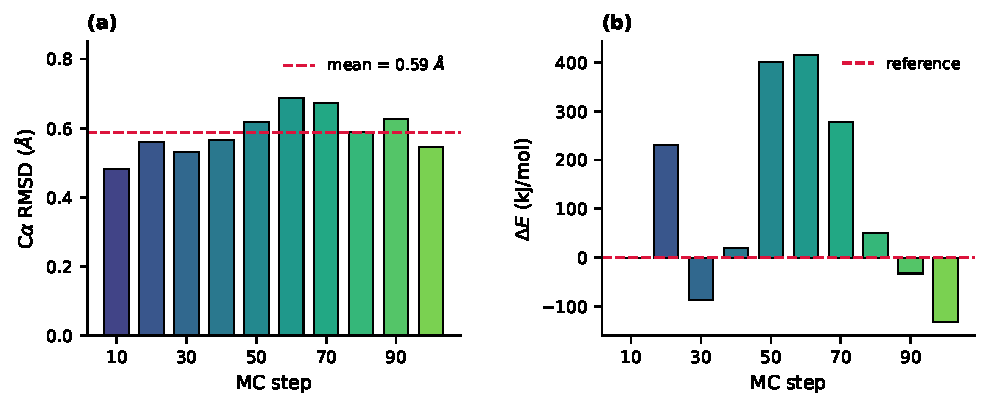
\includegraphics[width=0.72\linewidth]{fig_distributions_placeholder.pdf}%
  }{%
    \fbox{\begin{minipage}[c][0.28\textheight]{0.85\linewidth}\centering
    \vfill
    Place \texttt{fig\_distributions\_placeholder.pdf} in \texttt{docs/} to include the RMSD and energy panel.\\
    \vfill
    \end{minipage}}%
  }
  \caption{\textbf{Structural and energetic distributions of the unbiased TPS ensemble.}
  (a) C$\alpha$ RMSD of checkpoint structures relative to the first accepted structure
  (steps $10$--$100$). (b) OpenMM minimized energies (kJ/mol). Narrow RMSD spread
  indicates a sharply funneled denoising landscape for this input.}
  \label{fig:distributions}
\end{figure}

\subsection{Collective Variables for OPES and Diagnostics}

For the co-folding experiment, the two-dimensional OPES bias acts on
$\mathbf{s} = (s_1, s_2)$: $s_1$ is the ligand heavy-atom RMSD after Kabsch
alignment to a reference crystal pose (\AA), and $s_2$ is the ligand
center-of-mass to nearest binding-pocket C$\alpha$ distance (\AA) as
implemented in the repository. Small $s_1$ with moderate $s_2$ marks a
native-like basin; larger $s_1$ or shifts in $s_2$ track pose slippage and
pocket engagement changes. The published run used $\gamma = 10$, barrier
$5\,k_BT$, pace $1$, compression threshold $1.0$, ending with $1159$
depositions and $82$ compressed kernels.

The module \texttt{collective\_variables.py} logs additional geometry and
model-confidence scalars to \texttt{cv\_values.json} without feeding OPES:
contact order, steric clash counts, lDDT \citep{mariani2013lddt}, Ramachandran
outlier fractions, radius of gyration, Boltz mean pLDDT, and (for some
pipelines) OpenMM-relaxed C$\alpha$ RMSD. These are filters on plausibility and
memorization diagnostics, not terms in $P(\mathcal{X})$.

\subsection{TPS+OPES: Projected Landscape and Structures}

Figure~\ref{fig:opes2d} shows the three-panel summary (kernel mixture, a
reweighted free-energy proxy, and a visitation histogram) when
\texttt{docs/figs/opes\_tps\_ligand\_2d\_fes.png} is available. The dominant
peak near $(s_1, s_2) \approx (0.07~\mathrm{\AA},\,5.37~\mathrm{\AA})$ aligns
with the native-like basin; secondary structure near
$(0.70~\mathrm{\AA},\,5.55~\mathrm{\AA})$ and $(0.83~\mathrm{\AA},\,5.61~\mathrm{\AA})$
marks metastable pose basins at elevated ligand RMSD.

\begin{figure}[t]
  \centering
  \IfFileExists{figs/opes_tps_ligand_2d_fes.png}{%
    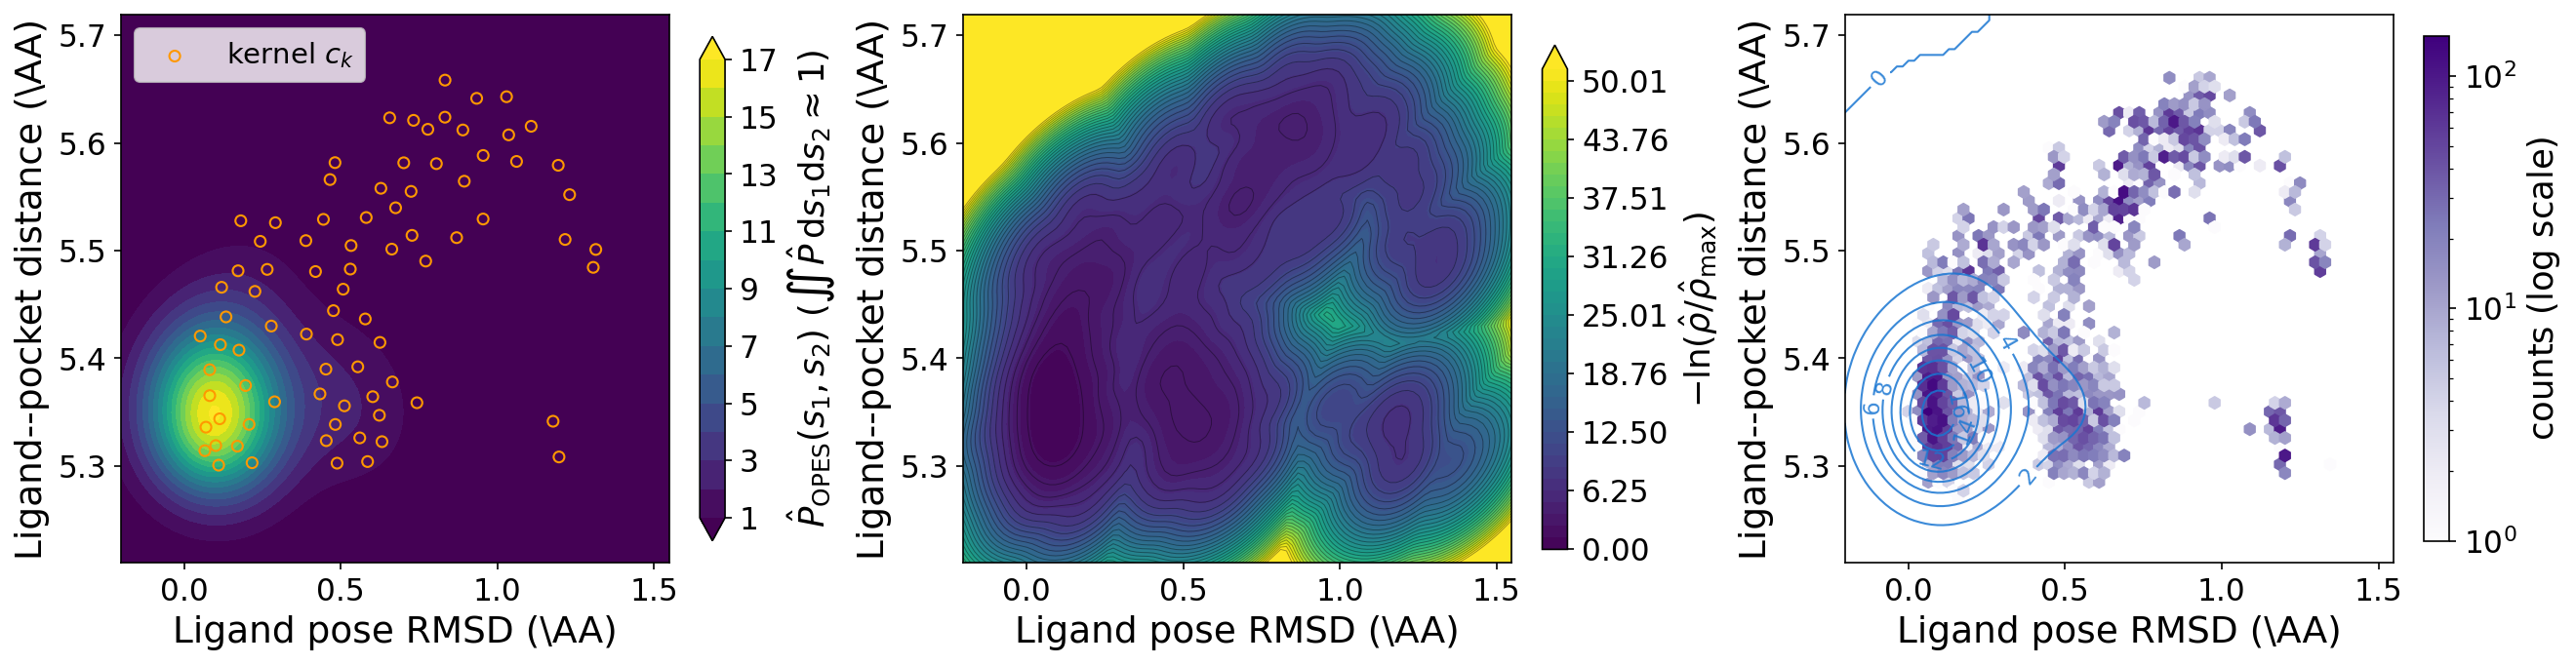
\includegraphics[width=0.92\linewidth]{figs/opes_tps_ligand_2d_fes.png}%
  }{%
    \fbox{\begin{minipage}[c][0.32\textheight]{0.9\linewidth}\centering
    \vfill
    Place \texttt{figs/opes\_tps\_ligand\_2d\_fes.png} under \texttt{docs/figs/} to include the triptych.
    \vfill
    \end{minipage}}%
  }
  \caption{\textbf{OPES--TPS two-dimensional summary in ligand pose space.}
  Kernel mixture, reweighted free-energy proxy, and visitation histogram with
  overlaid OPES contours (see repository scripts for regeneration).}
  \label{fig:opes2d}
\end{figure}

\begin{figure}[t]
  \centering
  \IfFileExists{figs/basin_structural_ensemble.png}{%
    \includegraphics[width=\linewidth]{figs/basin_structural_ensemble.png}%
  }{%
    \fbox{\begin{minipage}[c][0.35\textheight]{0.9\linewidth}\centering
    \vfill
    Place \texttt{figs/basin\_structural\_ensemble.png} under \texttt{docs/figs/} for basin-resolved structures.
    \vfill
    \end{minipage}}%
  }
  \caption{\textbf{Basin-resolved structural ensemble from TPS+OPES.}
  Representative terminal structures from metastable basins in the
  two-dimensional projection (cf.\ Figure~\ref{fig:opes2d}).}
  \label{fig:structures}
\end{figure}

Representative snapshots (Figure~\ref{fig:structures}, when available) show
native-like packing in the dominant basin and progressively displaced ligand
poses in higher-$s_1$ basins with modest increases in $s_2$, consistent with
geometrically distinct pocket engagement rather than pure rigid-body copies.

\subsection{Marginal Statistics and Run-Length Behavior}

Table~\ref{tab:cv-stats} reproduces the summary from
\texttt{scripts/summarize\_opes\_2d\_cv.py} on \texttt{opes\_tps\_out\_case1\_2d}.

\begin{table}[t]
\centering
\caption{Marginal CV statistics for the OPES--TPS two-dimensional run (case~1). ``All'' includes every logged step; ``Acc.'' conditions on accepted moves.}
\label{tab:cv-stats}
\begin{tabular}{lcccccc}
\toprule
 & \multicolumn{3}{c}{Ligand RMSD $s_1$ (\AA)} & \multicolumn{3}{c}{Pocket distance $s_2$ (\AA)} \\
\cmidrule(lr){2-4}\cmidrule(lr){5-7}
Subset & Mean $\pm$ SD & Median & $p_{95}$ & Mean $\pm$ SD & Median & $p_{95}$ \\
\midrule
All  & $0.49 \pm 0.35$ & $0.49$ & $1.19$ & $5.44 \pm 0.11$ & $5.40$ & $5.62$ \\
Acc. & $0.38 \pm 0.32$ & $0.26$ & $0.95$ & $5.41 \pm 0.10$ & $5.37$ & $5.61$ \\
\bottomrule
\end{tabular}
\end{table}

Among all logged steps, $48.9\%$ have $s_1 > 0.5$~\AA, $23.5\%$ exceed
$0.75$~\AA, $8.8\%$ exceed $1.0$~\AA, and $1.7\%$ exceed $1.25$~\AA.
Accepted paths show lower tail mass at the same thresholds ($36.6\%$,
$14.7\%$, $4.5\%$, $0.9\%$), reflecting the tension between OPES steering toward
high RMSD and the Metropolis filter that still favors paths with reasonable TPS
weights.

Run-length analysis on the stored chain shows that excursions with
$s_1 > 0.5$~\AA\ appear in sustained segments (mean length $39$ steps, maximum
$299$ over all logs), rather than isolated spikes. On accepted steps alone, the
mean run length above the same threshold is about $8$, still indicating
metastable dwell rather than single-point noise.

These empirical findings motivate the interpretation and limitations discussed
next.

\section{Discussion}
\label{sec:discussion}

The experiments in Section~\ref{sec:experiments} support a consistent
qualitative picture for the studied input: Boltz-2's reverse diffusion under
the reported configuration behaves like a sharply funneled stochastic map
toward a dominant terminal basin, while TPS+OPES still surfaces persistent
excursions to elevated ligand RMSD at non-negligible frequency along the biased
chain. Interpreting those excursions requires separating three issues: (i) what
the \emph{unbiased} path measure says about concentration; (ii) what a
two-dimensional OPES projection reveals about a \emph{margin} of the path
measure; and (iii) how much of the tail is attributable to adaptive bias updates
versus genuine secondary basins of the underlying generator.

\paragraph{Sharp funnel versus memorization.}
A single forward pass cannot distinguish a sharply legitimate ensemble from an
overly rigid memorized map. Unbiased TPS is designed to answer that distinction
at the path level: if the induced path measure were diffuse, accepted paths
would explore structurally diverse terminals at appreciable rates under the
same move set. The observed sub-angstrom RMSD spread instead indicates that,
for this input, most stochastic mass sits near one binding geometry. That
conclusion is not a sampling artifact of forward shooting: each accepted path
involves independent draws of augmentation and churn noise, so identical
terminal packing reflects the generator rather than a failure to perturb the
chain.

\paragraph{OPES projections and caveats.}
The two-dimensional OPES summaries should be read as biased-path statistics
together with the fixed-bias lemma (Lemma~\ref{lem:opes-mh}) and the adaptive-bias
remark in Section~\ref{sec:opes-theory}. Different $(\gamma, \mathrm{barrier},
\mathrm{pace})$ choices change the visited kernel mixture and therefore the
shape of reported surfaces. Secondary peaks can also arise from projection:
distinct three-dimensional configurations can map to similar $(s_1,s_2)$.
Cross-checking with diagnostic scalars logged alongside trajectories (clashes,
Ramachandran outliers, lDDT, pLDDT) remains essential before chemical
interpretation.

\paragraph{Generality.}
The same TPS construction applies to other generators cast as explicit
discrete-time Markov kernels with tractable noise priors, including many
score-based samplers and flow-matching implementations \citep{lipman2022}. The
Boltz-2-specific content is the map $T_i$, the schedule, and the augmentation
stack; Sections~\ref{sec:kernel-full}--\ref{sec:diffusion-boltz} document that
specialization pattern for reuse.

\paragraph{Relation to Boltzmann generators and action methods.}
Deep equilibrium models trained as Boltzmann generators define path measures
similar to Eq.~\eqref{eq:forward-kernel-product} and have been combined with TPS
for rare events \citep{falkner2023}. Complementary approaches interpret
diffusion as inducing dynamics whose likely paths minimize an action functional
\citep{raja2025omtps}. Our emphasis is diagnostic rather than control: we use
exact MH corrections for the given pretrained sampler rather than learning a
new path measure.

Section~\ref{sec:conclusion} collects practical takeaways and open directions.

\section{Conclusion and Future Work}
\label{sec:conclusion}

We cast the Boltz-2 reverse sampler as a discrete-time Markov chain on an
extended path space, derived the associated path measure and Metropolis--Hastings
moves (including backward shooting and global reshuffle), analyzed Jacobian
diagnostics in the extended-variable parameterization, and combined TPS with
OPES bias on terminal-frame collective variables. On a $228$-residue
protein--ligand co-folding example without MSA, unbiased TPS shows a concentrated
terminal ensemble, while TPS+OPES exposes additional pose basins in a
two-dimensional ligand projection.

Natural extensions include varying MSA depth to test how evolutionary
information reshapes path-level concentration; sweeps over OPES hyperparameters
with reweighting checks; learned or nonlinear collective variables
\citep{invernizzi2022}; and porting the same path MCMC stack to additional
public structure generators for comparative diagnostics.

\paragraph{Reproducibility.}
The LaTeX source, sampling scripts, and analysis utilities for the figures and
tables in Section~\ref{sec:experiments} are maintained in the project
repository (\texttt{tps-diffusion-model}) alongside frozen configuration files
for the reported runs.


\acks{The author acknowledges support from the Simons Center for Computational
Physical Chemistry (SCCPC) at New York University (SF Grant No.~839534) and
the use of NYU IT High Performance Computing resources.}

\bibliography{si_refs}

\end{document}
